\documentclass[conference]{IEEEtran}
\renewcommand{\refname}{Referências}
\IEEEoverridecommandlockouts
\usepackage{cite}
\usepackage{amsmath,amssymb,amsfonts}
\usepackage{algorithmic}
\usepackage{graphicx}
\usepackage{textcomp}
\usepackage{xcolor}
\usepackage{float}
\usepackage[utf8]{inputenc}
\usepackage[T1]{fontenc}
\usepackage[portuguese]{babel}

\def\BibTeX{{\rm B\kern-.05em{\sc i\kern-.025em b}\kern-.08em
    T\kern-.1667em\lower.7ex\hbox{E}\kern-.125emX}}
\begin{document}

\title{Binarização Híbrida de Imagens de Documentos Históricos Degradados: Uma Releitura Adaptada\\
{\footnotesize }
}

\author{\IEEEauthorblockN{Vitor Guedes Frade - 221017130 \\ Ryan Reis Fontenele - 211036132 \\ Mateus Elias de Macedo - 222011561}
\IEEEauthorblockA{\textit{Departamento de Ciências da Computação} \\
\textit{Universidade}\\
Brasilia, Brasil \\
vitorguedesfrade@gmail.com \\ 
ryanreisfonte@gmail.com  
\\ mateus.emacedo@gmail.com
}
}

\maketitle

\selectlanguage{english}
\begin{abstract}
This paper presents a reinterpretation and adaptation of a hybrid system for binarizing degraded historical document images. Based on techniques established in the literature, the implemented method integrates pre-processing, dynamic global binarization, adaptive local binarization, and morphological post-processing. Adaptations were made to the original method to improve results, substituting some approaches with optimized implementations, such as Multi-Otsu and Hit-Miss morphology. Parameter adjustments diverging from the base article were empirically chosen to better suit the specific degradation profiles of our test set. The results demonstrate the algorithm's efficacy in preserving writing strokes in low-contrast regions and mitigating background noise, smear, and unwanted artifacts.
\end{abstract}

\begin{IEEEkeywords}
Image Processing, Hybrid Binarization, Historical Documents, Otsu, Nick's Method, CLAHE, Mathematical Morphology.
\end{IEEEkeywords}
\selectlanguage{portuguese}

\section{Introdução}
A binarização de imagens de documentos é uma etapa primordial e crítica em muitos sistemas de análise e reconhecimento de documentos. O processo de separação entre os objetos pertinentes (texto) e o fundo do documento é frequentemente dificultado por degradações comuns em documentos históricos, tais como iluminação não uniforme, manchas, variações no contraste e caracteres desbotados.

Este trabalho consiste na reprodução e adaptação da metodologia proposta por Boudraa et al. (2019) \cite{boudraa2019}, que sugere um sistema de binarização em múltiplas fases (pré-processamento, binarização híbrida e pós-processamento). No entanto, para fins de melhoria de desempenho e adequação das ferramentas disponíveis, foram implementadas modificações estratégicas na lógica de limiarização global e nas operações de pós-processamento, buscando resultados superiores no tratamento de ruídos e artefatos específicos das imagens utilizadas no conjunto de testes.

\section{Metodologia e Adaptações}
O desenvolvimento foi conduzido em ambiente Python. O algoritmo foi estruturado nas seguintes etapas, com divergências metodológicas e de parametrização em relação ao artigo base justificadas a seguir:

\subsection{Pré-Processamento e Análise de Contraste}
Para tratar imagens com iluminação deficiente, implementou-se uma etapa de análise de contraste local de Michelson (núcleo $3\times3$). A média global desse mapa de contraste dita a aplicação do CLAHE. O limite de aplicação (contraste médio $< 0,02$) foi mantido como um estimador robusto para imagens altamente desbotadas.

\subsection{Limiarização Global Dinâmica (Divergência TSMO vs. Multi-Otsu)}
Diferentemente do método TSMO original sugerido pela literatura base, esta releitura adota o algoritmo Multi-Otsu (com 3 classes) em conjunto com o Otsu padrão. A decisão sobre qual limiar utilizar baseia-se diretamente no valor do contraste local médio calculado na etapa anterior, utilizando três faixas de restrição empíricas ($T_{01} = 0,03$, $T_{02} = 0,04$ e $T_{03} = 0,085$). 

Esses parâmetros foram ajustados empiricamente para a nossa base de testes, pois os intervalos originais sugeridos no artigo base geravam perdas acentuadas na continuidade dos traços em imagens com contraste marginal. A lógica de decisão estruturada ocorre sob as seguintes faixas:

\begin{itemize}
    \item \textbf{Contraste Extremo Baixo ($\le T_{01}$):} Utiliza o limiar superior do Multi-Otsu.
    \item \textbf{Contraste Muito Baixo ($\le T_{02}$):} Analisa a densidade de pixels na faixa intermediária e a distância entre os limiares. Caso atenda às condições restritivas, adota-se o limiar superior do Multi-Otsu; caso contrário, o Otsu clássico.
    \item \textbf{Contraste Moderado ($\le T_{03}$):} Aplica a limiarização clássica de Otsu.
    \item \textbf{Contraste Alto ($> T_{03}$):} Utiliza o limiar inferior do Multi-Otsu para evitar ruídos de fundo.
\end{itemize}

\subsection{Limiarização Local Adaptativa de Nick}
Para tratar as áreas onde a binarização global falha (textos desbotados e manchas), implementou-se o método adaptativo de Nick:
\begin{equation}
T(x,y) = m + k_{nick} \sqrt{\frac{\sum (p_i^2) - m^2}{N}}
\end{equation}
\textbf{Justificativa do Parâmetro:} O artigo base e a literatura frequentemente sugerem valores de $k_{nick}$ entre $-0,1$ e $-0,2$. Neste trabalho, optou-se pelo valor divergente $k_{nick} = -0,05$ e janela $ws = 7$. Um valor absoluto menor de $k$ torna o limiar menos agressivo. Isso foi intencional: visou-se preservar mais informações dos traços do texto em áreas severamente manchadas, assumindo o risco de manter algum ruído residual, o qual é agressivamente tratado e eliminado na nossa etapa otimizada de pós-processamento (Hit-Miss).

\subsection{Detecção de Manchas e Mesclagem Híbrida}
O algoritmo subdivide a imagem binarizada globalmente em blocos não sobrepostos de $7\times7$. Se a fração de pixels pretos excede $\mu + k_{smear}\sigma$, a região é classificada como mancha. O valor escolhido de $k_{smear} = 0,001$ difere do habitual estatístico (que seria mais conservador) para aumentar a sensibilidade da detecção de manchas (smears), forçando o algoritmo a usar o método de Nick em praticamente qualquer região suspeita de acúmulo de tinta.

\subsection{Pós-processamento Morfológico Hit-Miss e Filtragem de Componentes}
O artigo base sugere algoritmos de pós-processamento baseados em regras geométricas complexas para a limpeza da imagem. Nesta releitura, essa abordagem foi substituída por um conjunto de operações morfológicas via transformada \textit{Hit-Miss} aliada a uma rigorosa filtragem de componentes conexos, modificação escolhida por apresentar resultados superiores e maior robustez na limpeza de ruídos no nosso contexto de testes. As etapas projetadas para detecção e mitigação de anomalias são:

\begin{enumerate}
    \item \textbf{Gaps e Dots (Pontos isolados e Buracos):} Remoção de falsos pixels de \textit{foreground} e preenchimento de pequenos buracos no texto utilizando matrizes específicas da transformada \textit{Hit-Miss}.
    \item \textbf{Filtragem por Componentes Conexos (Substituição do Método Base):} Em vez das múltiplas etapas de verificação de vizinhança propostas na literatura original, adotou-se a remoção direta baseada em área. O algoritmo analisa todas as componentes e remove sumariamente aquelas com áreas inferiores a um limite estatístico restritivo $(\lambda \cdot \mu) / \sigma$, com $\lambda = 45$. Esta alteração substitui as regras originais por se mostrar muito mais eficaz na eliminação do ruído residual denso, especialmente aquele gerado pela limiarização de Nick nas áreas de manchas.
    \item \textbf{Convexidades e Concavidades:} Foram criados bancos de kernels (Cima, Baixo, Esquerda, Direita) para suavizar o contorno dos caracteres, subtraindo convexidades de 1 pixel e adicionando concavidades.
\end{enumerate}
\section{Resultados e Discussão}
O método proposto foi testado na base de imagens apresentada. O cálculo de contraste local aliado à decisão condicional entre Otsu e Multi-Otsu mostrou-se computacionalmente mais leve e eficiente que o TSMO original para as imagens do conjunto de dados.

A Figura \ref{fig:h05} ilustra perfeitamente a necessidade da binarização híbrida e o papel crucial da binarização de Nick nas manchas (smear). Na binarização puramente global (Fig. \ref{fig:h05}b), grandes áreas de acúmulo de tinta ou variação de iluminação colapsam em manchas densas, ocultando completamente o texto. Ao identificar essas regiões (densidade $> \mu + k_{smear}\sigma$) e aplicar localmente a fórmula de Nick com nosso $k_{nick}=-0,05$ otimizado (Fig. \ref{fig:h05}c), o texto é resgatado do fundo escuro. Por fim, o pós-processamento Hit-Miss (Fig. \ref{fig:h05}d) elimina os resíduos pontuais e preserva a integridade estrutural da escrita.

\begin{figure}[htbp]
    \centering
    \begin{minipage}{0.48\columnwidth}
        \centering
        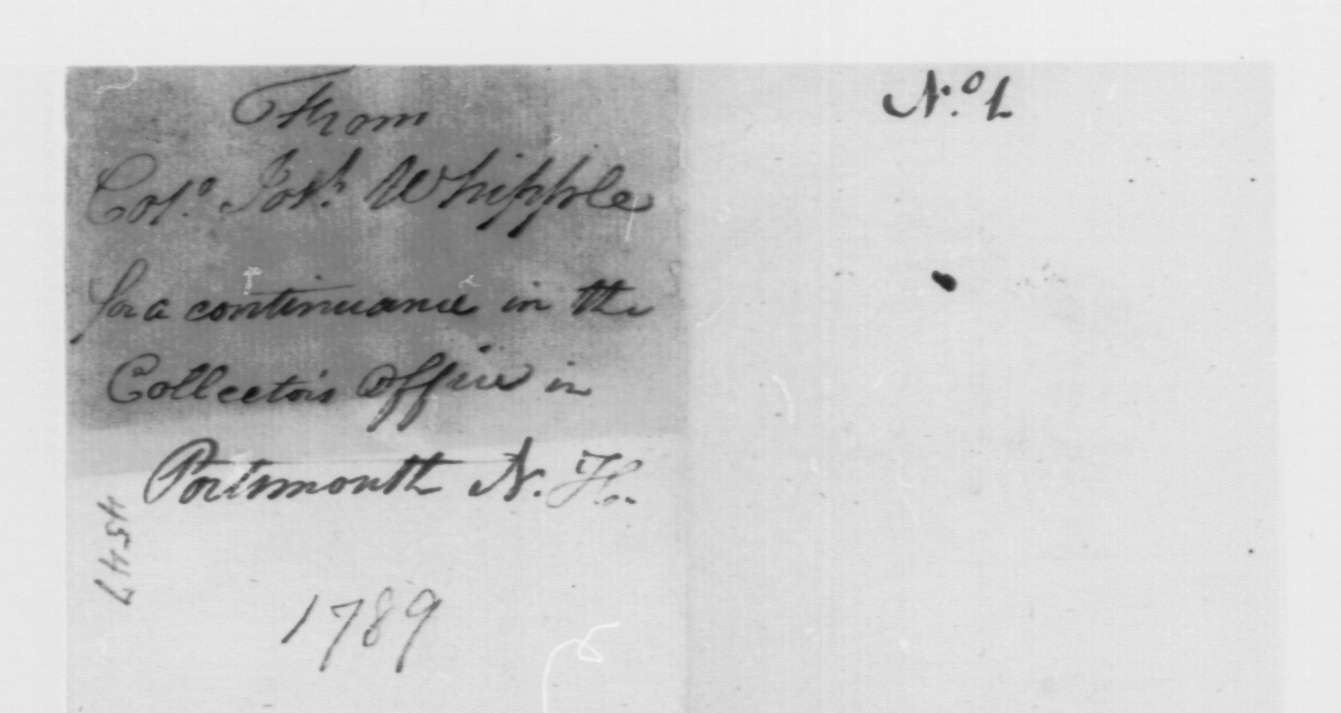
\includegraphics[width=\linewidth]{resultados_binarizacao_nick/H05_01_Original_Gray.png}
        \vspace{-0.2cm}
        \caption*{(a) Imagem Original}
    \end{minipage}
    \hfill
    \begin{minipage}{0.48\columnwidth}
        \centering
        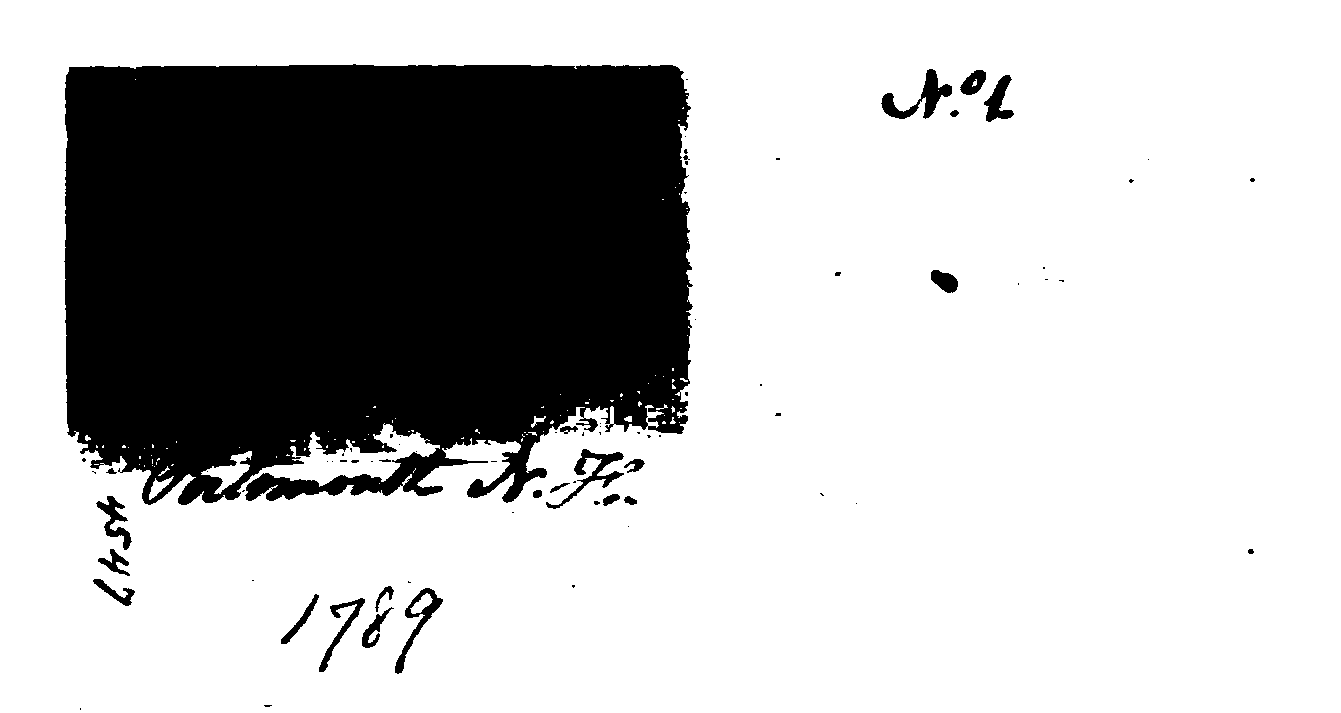
\includegraphics[width=\linewidth]{resultados_binarizacao_nick/H05_02_Binarizada_global.png}
        \vspace{-0.2cm}
        \caption*{(b) Binarização Global}
    \end{minipage}
    \vspace{0.3cm}
    
    \begin{minipage}{0.48\columnwidth}
        \centering
        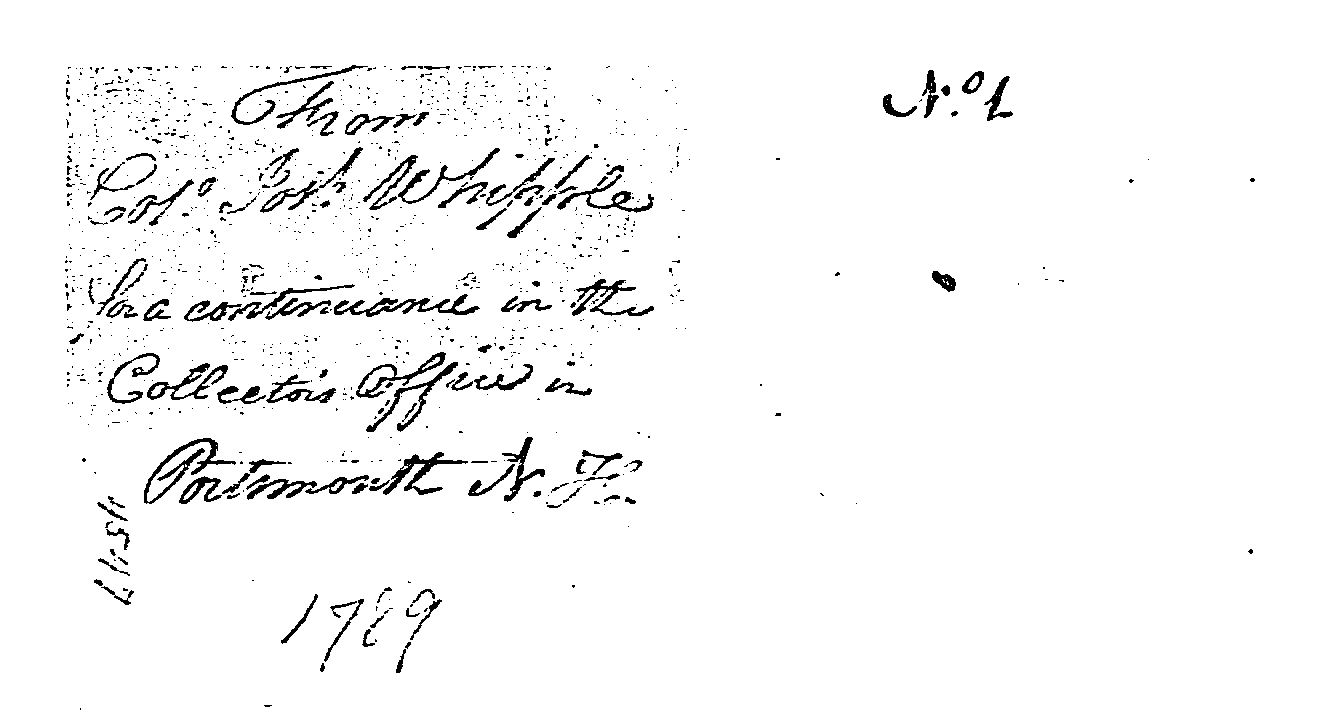
\includegraphics[width=\linewidth]{resultados_binarizacao_nick/H05_03_Binarizada_Nick.png}
        \vspace{-0.2cm}
        \caption*{(c) Binarização de Nick}
    \end{minipage}
    \hfill
    \begin{minipage}{0.48\columnwidth}
        \centering
        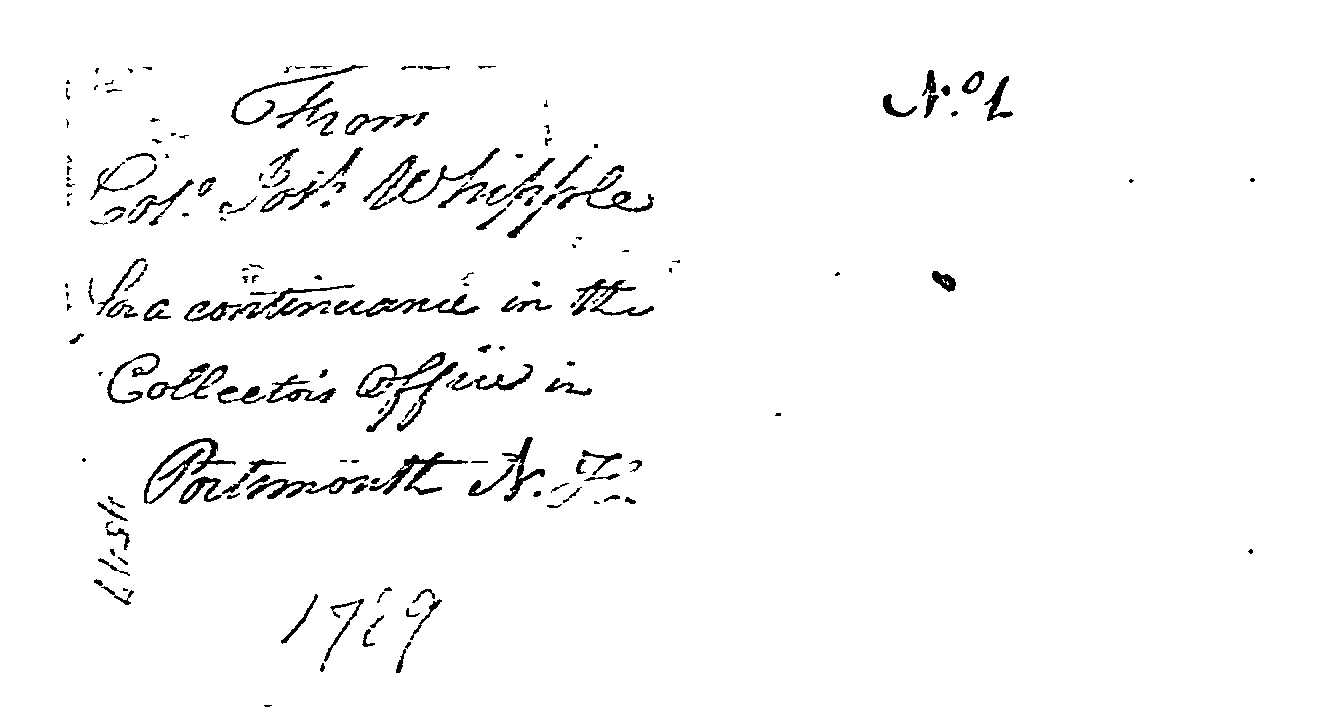
\includegraphics[width=\linewidth]{resultados_binarizacao_nick/H05_04_Pos_Processada.png}
        \vspace{-0.2cm}
        \caption*{(d) Final (Pós-processada)}
    \end{minipage}
    \caption{Comparativo das etapas na imagem H05. A binarização global (b) deixa manchas opacas devido à degradação. A aplicação da limiarização de Nick (c) nestas regiões recupera o texto, sendo o ruído residual limpo no pós-processamento (d).}
    \label{fig:h05}
\end{figure}

Caso o algoritmo fosse executado com os parâmetros sugeridos pelo artigo base (por exemplo, valores de $k_{nick}$ mais negativos e janelas maiores), notaríamos uma erosão excessiva dos caracteres resgatados nas áreas de mancha. A nossa parametrização compensa isso balanceando um $k_{nick}$ tolerante com uma limpeza morfológica posterior rigorosa. As imagens geradas pelo código permitem a validação visual dessas assunções perante a literatura base.

\section{Conclusão}
A releitura do sistema híbrido alcançou seus objetivos. A divergência consciente dos parâmetros (como no limiar de Nick e no limite estatístico de smear) combinada com a substituição do pós-processamento do artigo base por operações Hit-Miss, demonstrou ser uma adaptação extremamente eficaz. As evidências visuais comprovam a recuperação de informações essenciais em documentos gravemente manchados, consolidando a validade técnica das adaptações realizadas.

\begin{thebibliography}{00}
\bibitem{boudraa2019}
O. Boudraa, W. K. Hidouci, and D. Michelucci, ``Degraded Historical Documents Images Binarization Using a Combination of Enhanced Techniques,'' \textit{arXiv preprint arXiv:1901.09425}, 2019.
\end{thebibliography}

\end{document}
"""

with open("relatorio_releitura_v2.tex", "w", encoding="utf-8") as f:
    f.write(latex_content)

print("Fetched content: Successfully generated relatorio_releitura_v2.tex")
print("[file-tag: relatorio_releitura_v2.tex]")